\documentclass[12pt,journal,compsoc]{IEEEtran}

\usepackage{listings}
\usepackage{color}
\usepackage{graphicx}

\definecolor{dkgreen}{rgb}{0,0.6,0}
\definecolor{gray}{rgb}{0.5,0.5,0.5}
\definecolor{mauve}{rgb}{0.58,0,0.82}

\lstset{frame=tb,
  language=Java,
  aboveskip=3mm,
  belowskip=3mm,
  showstringspaces=false,
  columns=flexible,
  basicstyle={\small\ttfamily},
  numbers=none,
  numberstyle=\tiny\color{gray},
  keywordstyle=\color{blue},
  commentstyle=\color{dkgreen},
  stringstyle=\color{mauve},
  breaklines=true,
  breakatwhitespace=true,
  tabsize=3
}
   
\begin{document}

\title{Creating Situational Awareness of Location and Surroundings on a Campus}

\author{Liam J. Kelly}
        
\IEEEcompsocitemizethanks{\IEEEcompsocthanksitem L. Kelly is a student in the department of Electrical Engineering and Computer Engineering at Vanderbilt University, Nashville, TN 37235. E-mail: liam.j.kelly@vanderbilt.edu}% <-this % stops a space}

\markboth{EECE 6356 Intelligent Systems and Robotics Fall 2018}%
{Shell \MakeLowercase{\textit{et al.}}: Bare Advanced Demo of IEEEtran.cls for Journals}

\IEEEtitleabstractindextext{%
\begin{abstract}
Smartphones have become ubiquitous and come equipped with a wide array of sensors. Individually, each sensor has its own use, but by combing sensors, known as sensor fusion, noise can be mitigated and new insights can be made. Magnetometers and accelerometers can be used together to estimate the orientation of a body. In particular, one can estimate the orientation of a smartphone camera. Combining this information with GPS data, which can be corrected through a Kalman Filter, with prior knowledge of scenery, one can estimate what is seen by the camera. An example application of this is shown through the app 'Dore-Tours', which informs users of what they are looking at and where they are on a campus.
\end{abstract}

\begin{IEEEkeywords}
Sensor Fusion, Kalman Filter, YOLO Detection, Augmented Reality
\end{IEEEkeywords}}

\maketitle

\IEEEdisplaynontitleabstractindextext

\IEEEpeerreviewmaketitle



\section{Introduction}


\IEEEPARstart{I}{t} is a common dilemma for any individual new to a campus of figuring out where they are. Even with the assistance of applications such as Google Maps, determining one's orientation can be difficult, especially when buildings are clustered closely together. 

We have overcome this dilemma with promising results by creating an application which informs the user of when they are on a campus, which building they are in on that campus if they are in a building, and if they are not in a building, what building they are looking at, if any.  

\subsection{Obtaining Parameters}

The necessary parameters for the location detection and building recognition are GPS location, camera orientation, and images of buildings. While obtaining images of buildings only requires using Android hardware APIs, obtaining the other two accurately is a non-trivial problem.

\subsubsection{Obtaining GPS Data}

GPS data can be obtained from an Android API. However, GPS data is known to lack accuracy, with civilian GPS often accurate to about 4.9m \cite{gps_accuracy}. However, this can be corrected through a technique known as Kalman filtering. Kalman filters use Bayesian probability to recursively estimate a value. Because latitude and longitude are essentially the output of a 2D function, they can be treated as a single variable, meaning the Kalman filter can be implemented in 1-D. 

The mathematics of the Kalman filer involve a prediction step followed by an update step. The prediction step predicts the update of the tracked variables, in this case latitude and longitude, and their covariance, which in this case is simply their variance. This can be a fairly sophisticated step that considers how the variables' values change over time as well as how a 'control vector', or a force controlled by the actor may affect them. The accuracy of the measurement is considered and used to further affect the prediction of the covariance, or the error. A higher covariance suggests an inaccurate measurement. This becomes relevant in the update step, when the covariance is used to compute the Kalman gain. A higher covariance leads to a lower Kalman gain, meaning the difference between the measured value and the predicted value will be taken less into account since it is unreliable. On the other hand, a high Kalman gain suggests that the measured value is reliable, and the difference between it and the predicted value should be weighted more heavily. 

As noted, the Kalman filter used was quite simple because it was a 1-D case without a control vector. The code for prediction and update upon a new measurement is shown below:

\begin{lstlisting}

long currentTime = System.nanoTime();
long deltaTime = currentTime - mLastTimeNanoseconds;
mLastTimeNanoseconds = currentTime;
mVariance += PROCCESS_ERROR_COVARIANCE * PROCCESS_ERROR_COVARIANCE * deltaTime / 1000000000.0;
double kalmanGain = mVariance / (mVariance + (accuracy * accuracy));
for (int i = 0; i < mMeasurement.length; i++) {
    mVariable[i] += kalmanGain * (mMeasurement[i] - mVariable[i]);
}
mVariance = (1 - kalmanGain) * mVariance;
        
\end{lstlisting}

The Kalman Filter was implemented as a class used by a singleton class which provided GPS data throughout the app.

\subsubsection{Camera Orientation}

The raw data used for determining the orientation of the camera was accelerometer and magnetometer data. An android hardware API provided these, and it also offered an API for fusing them to calculate yaw, pitch, and roll. From these, a rotation matrix could be constructed. This rotation matrix was applied to the negative azimuthal unit basis vector. The resultant vector's first two components were considered the magnitudes in the East and North, respectively, while the third component was azimuthal. 

\subsection{Recognizing Locations and Buildings}

\subsubsection{Recognizing Locations}

GPS data was used to recognize whether an individual was on campus, and if so, whether that individual was also in a particular building. A campus was treated as a set of contours, while buildings were treated as single contours. In either case, to determine if an individual was within that contour, an algorithm discussed by W. Randolph Franklin \cite{polygon} was used to determine if the GPS location fell within that particular contour. The algorithm tests whether a point is inside a polygon. The idea behind the algorithm is to draw a ray from the point of question and count how many edges it crosses. If it crosses an even number of edges, then, if that number is non-zero, it must have crossed in and then out, meaning it must be outside. If it crosses an odd number of edges, then it must have crossed out, meaning it must be inside.

Whenever new GPS data arrived, a callback was invoked which ran this algorithm on the contours of a given campus. If it found the individual was on the campus, it would inform them on the screen, and then run the algorithm again on every building on that campus. If it was inside a building, it would display the name of that building on the screen, informing the user that they are inside it.

\subsubsection{Recognizing Buildings} 

Initially, recognizing buildings worked similarly to recognizing locations. Using the user's location as a starting point, 'steps' would be taken in the direction of the camera's orientation, so long as the camera was approximately held level such that a building could actually be in view. At each step, the algorithm used to determine location would be run on the updated GPS location to see if it had landed in a building. If it had, then it implied that the building was in the direction that the camera was oriented towards, and must be the building in view. The code for this algorithm is shown below:

\pagebreak

\begin{lstlisting}

public Building getBuildingInView(double northMagnitude, double 	eastMagnitude, double lat, double lon) {
    if (inCampus(lat, lon)) {
        for (Building building : mBuildings) {
            if (building.inBuilding(lat, lon)) {
                return building;
            }
        }
        lat += northMagnitude * VIEW_STEP_SIZE;
        lon += eastMagnitude * VIEW_STEP_SIZE;
        return getBuildingInView(northMagnitude, eastMagnitude, lat, lon);
    } else {
        return null;
    }
}
\end{lstlisting}

\begin{figure}
  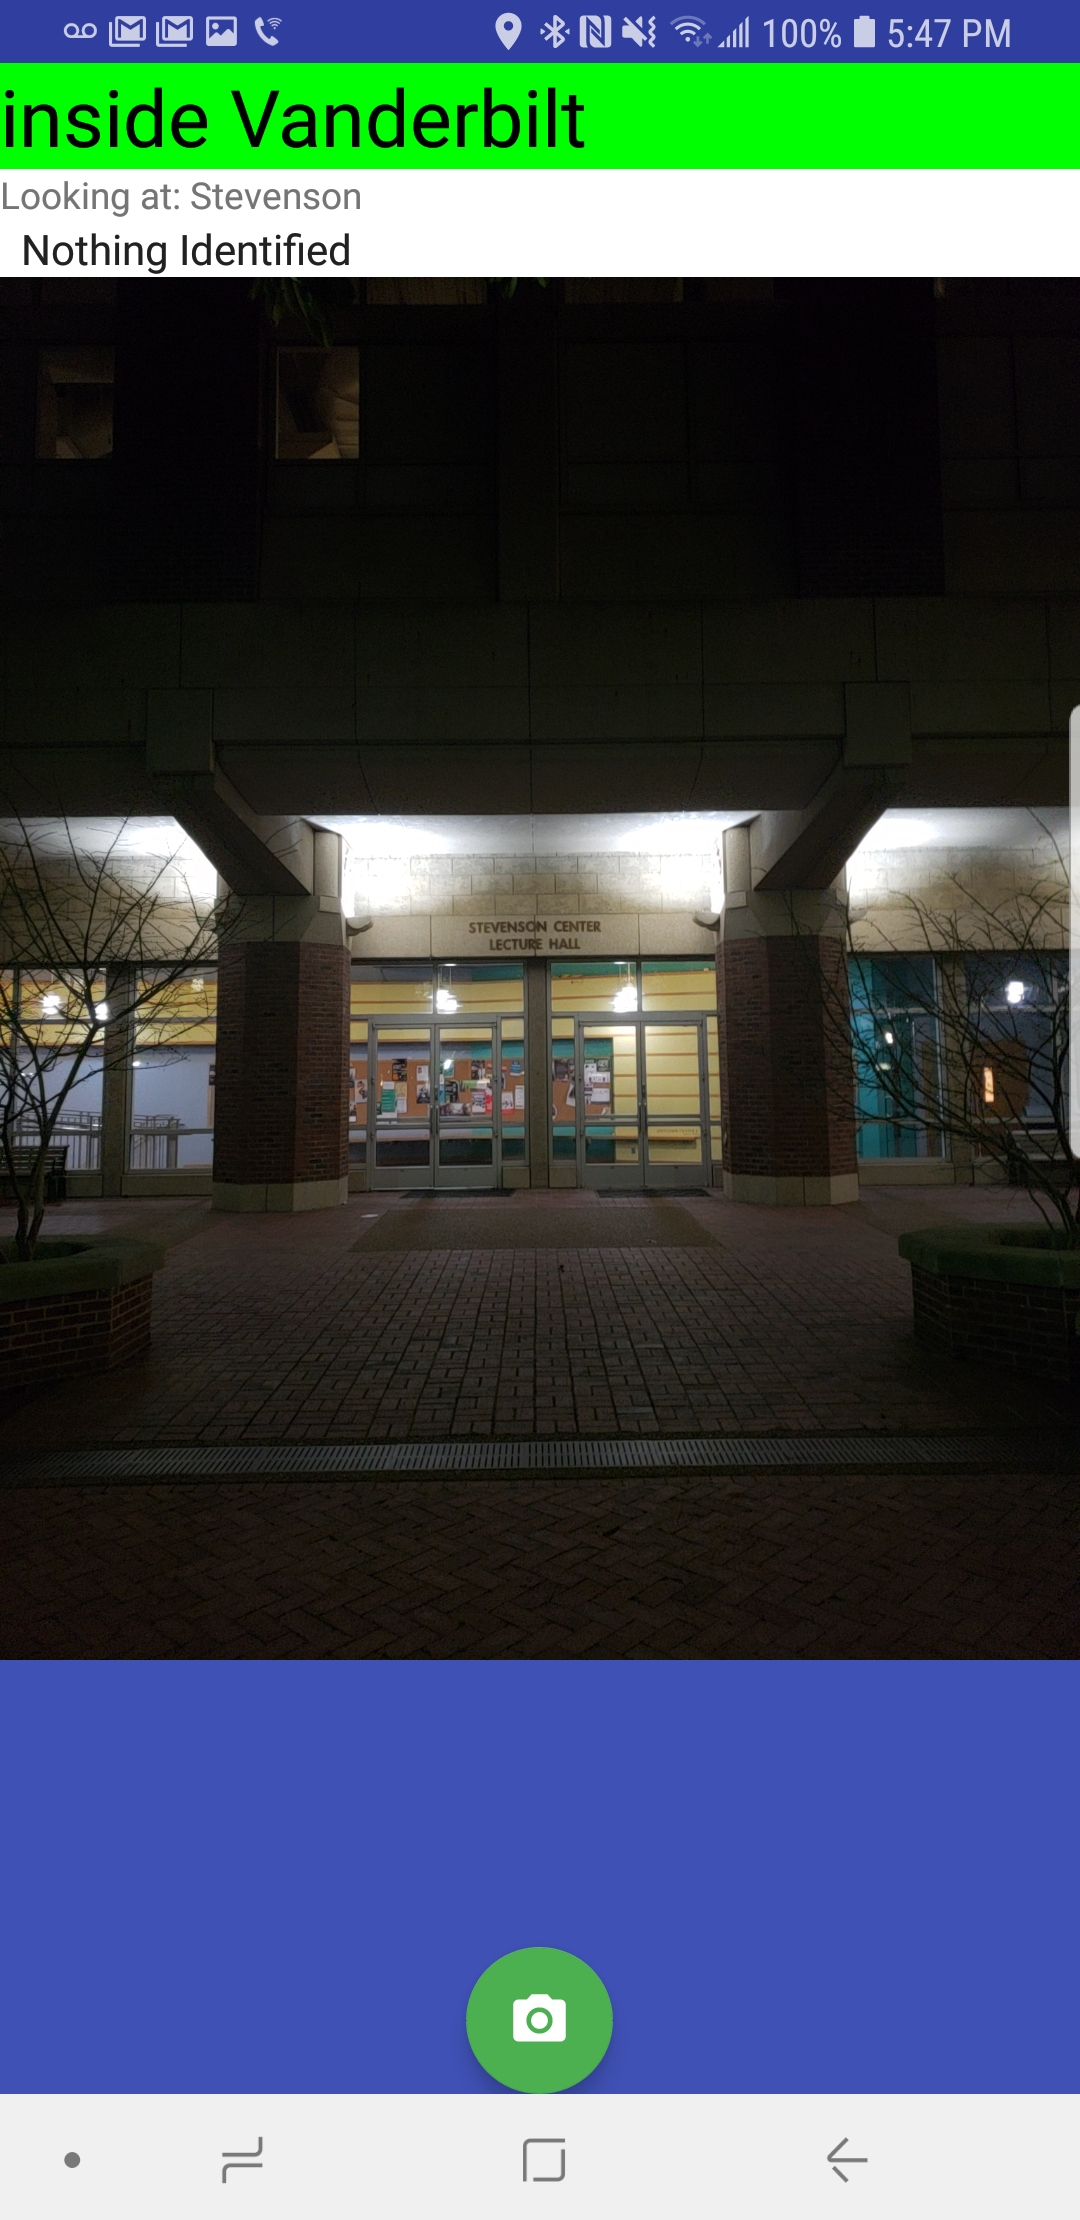
\includegraphics[width=\linewidth]{report_images/Stevenson.jpg}
  \caption{The app recognizing Stevenson.}
  \label{fig:stevenson}
\end{figure}

\subsection{YOLO Detection of Buildings}

A significant flaw with the GPS-step approach is that if the camera were pointed in the direction of a building far away, beyond sight, the phone would still inform the user that they were looking at that building, since the algorithm would keep taking steps in that direction until it hit that building.

A way to correct this is to determine if a building is actually within the image captured by the camera. This can be done with a YOLO detector, or a You-Only-Look-Once detector. This is an objector detection system which uses a neural net to create bounded boxes around objects which it has been trained on. Using a YOLO detector, the building recognition algorithm could be modified to only run if a building was in the image captured by the camera.

\subsubsection{Collecting Training Data}

To make collecting training data simpler, a pipeline was written which uploads captured images to the cloud. These images were labeled using the GPS-step recognition technique, as the result could be verified by the user before capturing the image and uploading. A script was written which pulled down the images and organized them into directories.

\subsubsection{Training the Neural Net}

Bounding boxes were drawn around the buildings using 

\subsection{Contouring Campuses}

As noted, the algorithms for determining location and what building is in view rely on contours of campus and buildings. These contours defined by vertices which are latitude-longitude pairs. To create contours more easily, a desktop application was written which leverages the Google Maps API. The application lets you search for a campus (e.g. "Vanderbilt University") and will then, if Google finds it, display the campus. There are buttons to zoom in and out and move around. Once a user is satisfied, they can draw contours on the screen with the mouse. These contours are pixels, but will be converted to latitude-longitude pairs using mercator projection. The contours are sampled so as not to create an excessive number of points in a contour, and then they are saved to a database. 

When the Android app starts, it will load available campuses, and upon selecting a campus, its buildings from the database.

\subsection{Future Work}

The intended user of the application is someone unfamiliar with their surroundings. To extend the functionality of this app, a proposed feature is to create augmented reality directions which are drawn on the app to guide a user to a destination building.

A limitation of the application is that because it relies on GPS, it cannot be used for guidance indoors. Another future potential extension of the app would be to create indoor maps that can be navigated through visual-inertial odometry.

\section{Conclusion}



\appendices
\section{Link to Source Code}
The source code for this project can be found at https://github.com/zappyfish/Dore-Tours


\ifCLASSOPTIONcompsoc
  \section*{Acknowledgments}
\else
  \section*{Acknowledgment}
\fi


The author would like to thank Professor Richard Alan Peters II for his guidance in project selection and development and for suggestions for this paper.

\ifCLASSOPTIONcaptionsoff
  \newpage
\fi

\begin{thebibliography}{9}

\bibitem{gps_accuracy}
\texttt{https://www.gps.gov/systems/gps/performance/accuracy}

\bibitem{polygon}
\texttt{https://wrf.ecse.rpi.edu/Research/Short\_Notes/pnpoly.html}

\end{thebibliography}

\end{document}



             